%************************************************
\chapter{Problems to Solve}\label{ch:problems_to_solve}
%************************************************

\section{Build a Reflective Knowledge Substrate}

The assumption that I introduced in
Section~\ref{sec:introducing_reflection_early_in_the_process},
``Introducing Reflection Early in the Process'', requires that changes
in my knowledge representation can be traced and compiled into other
representations, such as the reflective event representations used in
learning to accomplish goals.

\subsection{Automatic Collection of Audit Trails for All Processes}

Audit trails must be collected so that after the fact the events that
any process is resposible for can be used for many types of reflective
control purposes, such as learning to plan.  Although a system that
keeps track of everything that it does would support reflection, the
audit trail recorder in a system that does not grow indefinitely in
memory consumption would have options for focusing the collection of
audit trails, while also allowing for their garbage collection when
they are no longer needed by another reflective process.

\subsection{General Parallelism and Concurrency}

\begin{figure}[bth]
  \center
  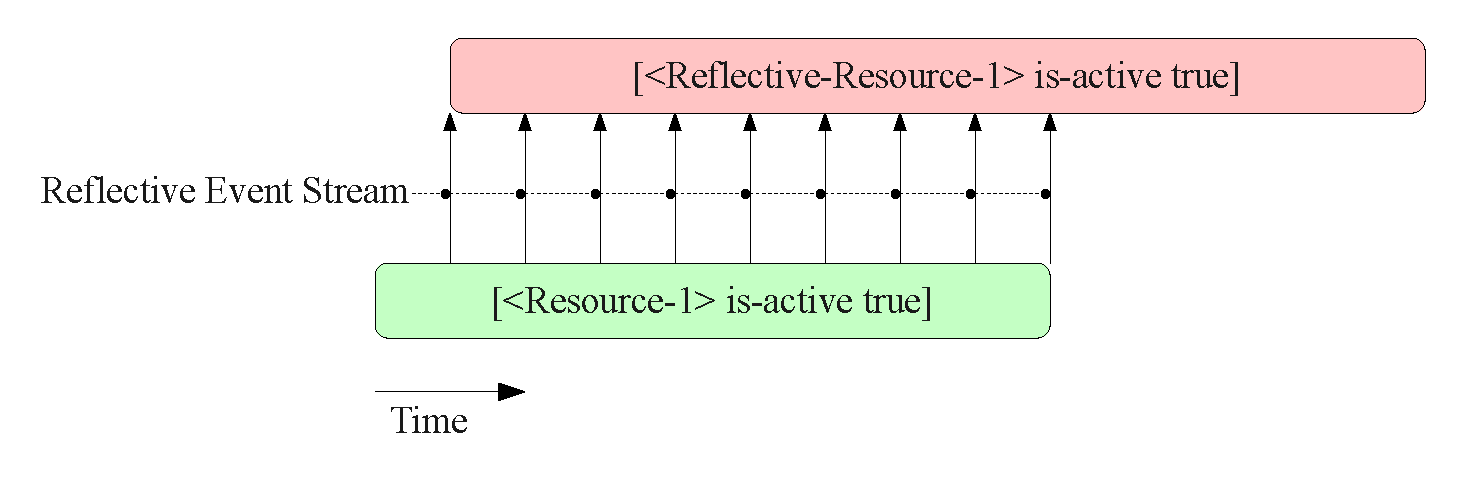
\includegraphics[width=11cm]{gfx/concurrent_parallel_reflection_efficiency}
  \caption[Concurrent parallel reflection efficiency]{Concurrent parallel reflection efficiency.}
  \label{fig:concurrent_parallel_reflection_efficiency}
\end{figure}

Because the procedurally reflective programming paradigm focuses on
event streams of changes to memory, there is an inherent ability to
express procedurally reflective algorithms in a streaming parallel
language.

Figure~\ref{fig:concurrent_parallel_reflection_efficiency} shows how a
simple process can be reflectively monitored without slowing down the
fundamental process by more than the constant time factor necessary
for generating the event stream.  Many different parallel reflective
processes can be reflectively processed concurrently without any
additional slowdown in the primary problem solving process.

\subsection{Program as Data}

The ability for a process to manipulate a program as data makes it
easier for that process or a user to read, edit, and write programs as
they are debugged.  The ability to change the functionality of a
program at run-time is a key component to creating an adaptive problem
solver.  Because of this, a programming language with a run-time
compiler is very useful for building these types of adaptive systems
that learn to debug and re-program their own subprograms.  For purely
the reason of developing problem solving learning algorithms, it is
critical that a reflective substrate has the ability to treat its own
programs as data.


\section{Layered Reflective Problem Solving}

\subsection{Analogy between Physical Goals and Planning Goals}


\section{Learning by Credit Assignment}

\subsection{Use Reflective Representations for Better Models of Learning}

\subsection{Tracing Knowledge Provenance for Credit Assignment of Success or Failure}



